\chapter{Results}

\begin{comment}
In this chapter I will present the results of my analysis.\\
Software:\\
Software engineering:\\
-what issues with the structure of different openMNGlab version did I encounter\\
-What are the needs of different users of the framework in the end?\\

Spike Analysis:\\
-Describe quantifiers and discuss the results of analysing the experimental recordings\\
-image of table containing everything the jupyter notebook has computed\\
-table with info on electrical frequency levels in each recording\\
-diagram showing a quantifier (peak firing frequency) and electrical frequency for each spike train of single recording\\
-compare diagrams of different recordings\\
-compare different quantifiers in one diagram with each other for the same file\\
-compare ISI to log(ISI) for every train in one file\\
\end{comment}


\section{Software}
\subsection{Data Structure}
I will begin by presenting the details of the different data structures that I will use in the course of my analysis pipeline.

\subsubsection{Neo Structure}
Neo models electrophysiological data in a hierarchical structure, which is depicted in figure~\ref{fig:neostructure}. On the lowermost level we start with different kinds of data objects. An \textit{AnalogSignal} is regularly sampled data and can contain multiple channels. An \textit{IrregularlySampledSignal} is similar, but does not feature a regular sampling interval. A \textit{SpikeTrain} object contains time point data with the information when action potentials occur. These \textit{SpikeTrain} objects can cover a large interval in time such as the whole duration of the recording and thus is a little different from the definition of a spike train that is otherwise used in this thesis, which I have described in the previous chapter. 
%The $SpikeTrain$ object in the Neo structure is a collection of all spikes during one recording and all spike trains as we see them would be contained in one such $SpikeTrain$ object.
\textit{Events} in Neo point to distinct points in time and can be used to mark stimulation events for experiments with animals for example. \textit{Epochs} function similar to events, but cover a duration instead of just points in time.

On the next layer up there are containers for grouping all of these lower level objects. The first of these containers is a \textit{Segment}. This groups data that was simultaneously recorded. On the topmost layer there are \textit{Blocks}. One \textit{Block} can contain multiple \textit{Segments} which in turn can contain multiple data objects.

In case of this Bachelor thesis we are dealing with recording files from animal experiments. When importing one such file, the resulting Neo structure looks as follows: On the top level each file contains a \textit{block}. In our case these \textit{blocks} contain only one \textit{segment}, since the recordings feature a single continuous signal without interruptions.

\begin{figure}
	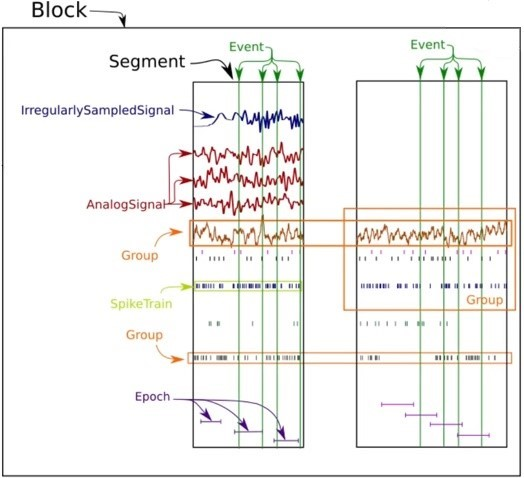
\includegraphics[width = \textwidth]{src/pic/neo_structure}
	\caption{An illustration of the data types supported by Neo and their grouping into containers.~\cite{neo14}. An \textit{AnalogSignal} and \textit{IrregularlySampledSignal} contains regularly and irregularly sampled data respectively. \textit{SpikeTrain} objects contain a set of spikes from the same source. \textit{Events} consist of a label and a time of occurrence and \textit{Epochs} represent a period of time in the experiment. The container object \textit{Segment} can contain multiple data objects that share the same clock. A \textit{Block} is the top-level container and can contain multiple \textit{Segments}.}
	\label{fig:neostructure}
\end{figure}

\subsubsection{Custom Structure}
The analysis notebook is still using code from version 1 from openMNGlab where the Neo structure was not yet integrated. The importer from version 1 delivered the data in a custom data structure.

At its core the custom data structure models the data hierarchically, but the objects look a little different from the ones from Neo. At the base level there are data objects \textit{ActionPotential}, \textit{MechanicalStimulus}, \textit{ElectricalStimulus} containing information corresponding to their respective names. These objects are all part of an overlying object type called \textit{signal\_artifact}.

On the top level we get an object called \textit{recording} when importing data with this method. One such \textit{recording} then contains the lists \textit{el\_stimuli}, \textit{mech\_stimuli}, \textit{actpots} which are lists containing objects of types \textit{ElectricalStimulus}, \textit{MechanicalStimulus} and \textit{ActionPotential} respectively. Additionally there is a \textit{raw\_signal} object which contains the raw signal in the form of arrays.


\subsection{Development Process}
To analyze any data a jupyter notebook is used which contains all the relevant code. I will now go over the stages in developing this notebook.
The base of the analysis notebook started with the work of Radomir Popovich, who also worked with spike train data for IMI. He had developed a jupyter notebook based on a custom import of spike train data extracted from the Spike2 software as a csv file. From this he extracted the spike trains and created figures such as event plots as seen in figure\ref{fig:eventplot}. This is a raster plot that depicts the spike trains of a single recording. Each row represents one spike train. The x axis represents the time since the last mechanical stimulus starting at 0. These figures give a good overview with one glance over the spiking activity during mechanical stimulation for recordings.
\begin{figure}
	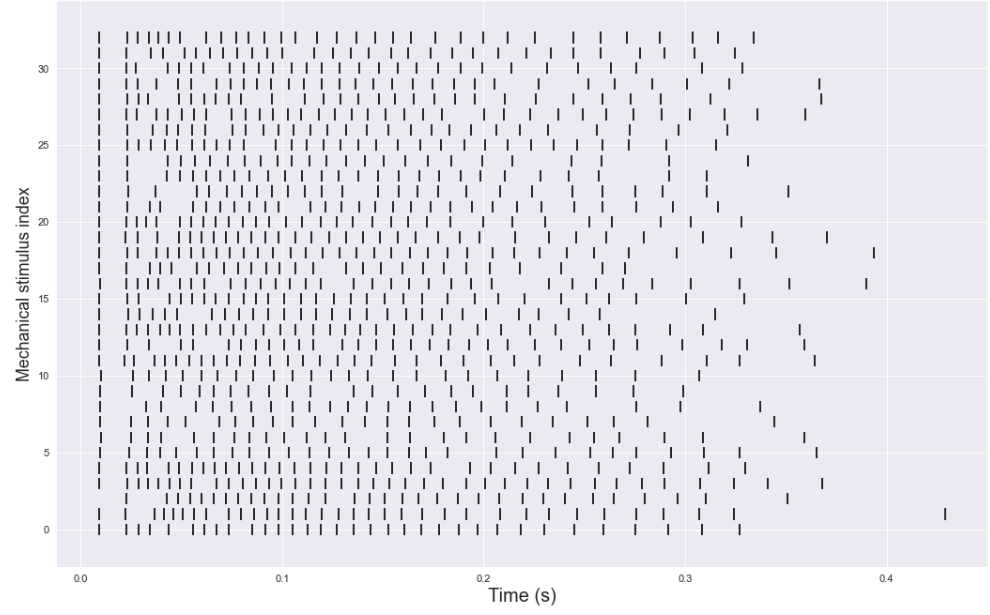
\includegraphics[width = \textwidth]{src/pic/event_plot}
	\caption{Event plot detailing spiking activity for one recording. The x axis notes the time since the start of the last mechanical stimulus. Each row on the y axis shows the spikes of one spike train. Each line represents one spike in the recording.}
	\label{fig:eventplot}
\end{figure}
Also included in this notebook was a way to filter the action potential channel so that only the relevant spikes for our spike trains remain. This was done by checking an interval of a specific duration after a mechanical stimulation event occurred for spikes and saving those in designated lists, which is still the method we use to extract the spike trains.

Starting from this point there were a couple of iterations trying to import the data, which can be seen in figure~\ref{fig:import_iteration}. The first iteration used the previously described custom import. The Spike2 data was exported into csv files that were then imported in the code. In addition version 1 of openMNGlab was used to import the spikes and mechanical events. This importing technique is rather slow, however, and is missing the electrical stimulation information, which is vital for the analysis.

When Neo was integrated into openMNGlab, it brought with it new ways of importing data. With this addition, the Spike2 files could be imported directly into the code, which resulted in fewer intermediate steps and is also much faster. The issue with the Neo importer of Spike2 data is that the spike sorting gets lost. The experimental researchers can apply spike sorting in the Spike2 software and create wavemark channels which feature only certain spikes. These channels do not get imported with the Neo importer and so the information which spikes are relevant and which spikes can be ignored gets lost. Another thing that is missing from the Neo import is the mechanical force channel. This means we are missing information about the duration and amplitude of the mechanical stimulus with this importing method.

In the end we combined all of the importing methods used in the previous two iterations. With the Neo import we gather the electrical events and stimulation frequency, with the custom import code from the very beginning the mechanical force channel is imported and with the import from version 1 of openMNGlab we receive the mechanical event timestamps as well as the spikes.

This is not an ideal solution, as three different importing methods are needed that result in three different data structures. The import of the csv file also slows down the analysis considerably, but for the purposes of this thesis and the analysis of only a few files this solution sufficed.
\begin{figure}
	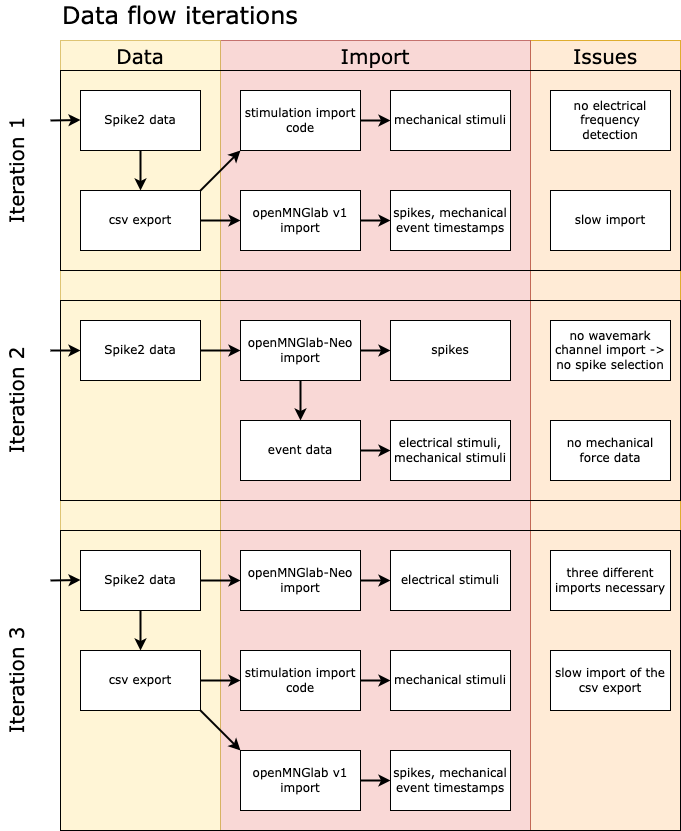
\includegraphics[width = \textwidth]{src/pic/Data_flow_iteration_vert}
	\caption{This diagram shows the different iterations that the data flow went through. The first iteration uses a custom csv import and the first version of openMNGlab to import mechanical stimuli and spikes. The second iteration uses the Neo importer from openMNGlab to import spikes and stimulus events. The third iteration combines the first two approaches to import spikes, electrical and mechanical stimuli.}
	\label{fig:import_iteration}
\end{figure}

%Add info about process with quantifiers
\subsubsection{Issues with importing and their Solutions}
%issues with nonworking files
%could not differentiate spikes from normal level of signal noise\\
There is a channel in the Spike2 files where experimenters can leave comments while experimenting. This is used to make notes on the experimental protocol of the recording in many cases. In the files that were provided for this thesis there were a couple of files where the character $\mu$ was contained in this channel. While importing the corresponding files an error appeared, because the importer did not recognize the Greek letters. This problem was circumvented by deleting the comment channels in those files, as they did not contain relevant information for my analysis. This is generally not a viable solution, since the comment channel is vital for many experiments and includes important information regarding the experimental conditions. Therefore, in the future openMNGlab needs to implement a fix to the importer, so that the comment channel can be included properly.

\begin{comment}
-Use-cases:\\
	\null\quad-opening data (importing)\\
	\null\quad-latency study (Alina)\\
	\null\quad-chemical data study (Jessica)\\
	\null\quad-mechanically evoked spike trains (Alexander)\\
	\null\quad-experimental researchers (Barbara)\\
-results in a list of requirements\\
-Use-cases lead to software engineering approach\\
-nessecary steps for my analysis\\
-how I implemented it
\end{comment}

\subsection{Use Cases}
To end the first part of this chapter I want to present a couple different use cases of various users of openMNGlab. I will describe the specifics of each use case and then give a few remarks on the current state of openMNGlab and the potential improvements necessary for a smoother experience for all users.

One important feature of openMNGlab that is needed in every use case is the importing of new data. For new users it is important to be able to load sample data sets and get a feel for the framework by getting to know a few test analysis functions. For students or experimental researchers it is key to be able to load multiple files for a quick overview or even full analysis.\\
Because we are dealing with a couple of different sources when it comes to experimental data, which all need to be handled in a different way, this is where many issues can occur. When going through the use cases we will see where already we encounter some difficulties regarding the data import.



\begin{comment}
-spike2 does some automatic spike filtering
-This results in up to 20 different classes of spikes in one recording
-not all of these, however, are in fact coming from different sources
-experimental researchers have already done their own filtering with their expertise, in order to combine various different of the spike2 classified spikes into larger groups and put them in so called wavemark channels.
-previously one could export these wavemark channels to csv files and inport those into the framework
-with the direct importer from the smr files, however, this is no longer possible
-what we receive after a successful import of an smr recording file are the original spike2 classified spikes in different channels
-if one were to know which of these belong together one could easily combine those together as in spike2 with the wavemark channels
-but the information of the wavemark channels is lost during the import and so one has to manually search for the correct channels first and then combine them into groups by hand
\end{comment}

\subsubsection{Student 1}
\begin{comment}
Alina \\
Works with spike2 data \\
Electrical data and mechanical data \\
Uses old way of importing currently (csv export from spike2) \\
Needed channels from csv export: \\
DigMark for electrical and mechanical stimulus events \\
WaveMark channel for timestamps of spikes \\
Information used: \\
Electrical stimulus events + timestamps \\
Calculate Latency for spikes (timestamps) \\
Calculate Spike Count  \\
In theory this information is available with the direct import of openMNGlab right now \\
Potential problems with direct openMNGlab importer: \\
Each template for spikes in spike2 results in separate channel in Neo structure after openMNGlab import -> needs some filtering (manual right now) \\
Electrical and mechanical events share a channel (DigMark) and somehow need to be distinguished if the recording also features mechanical stimulation \\
\end{comment}

The first user is a student who does data analysis on mechanically and electrically stimulated Spike2 data. The goal is to perform latency analysis for spikes.  The raw spike2 files feature a lot of information, not all of which is always needed. In this case, all that is required to analyze the latencies of the spikes are the timestamps of the spikes itself and the timestamps of the stimulation events. For the Spike2 software this means that we need to extract the DigMark channel which contains the event information as well as the corresponding wavemark channel which contains the information on the already presorted spikes.\\
The relevant information can be imported using the importing function of openMNGlab. 
The data is then used to calculate the latency for the spikes corresponding to the latest electrical stimulus event as well as calculating the spike count.

Potential problems: The student started the analysis before the framework was working properly and therefore uses their own custom analysis notebook. However, all the information that is required is also available with the regular Spike2 importer in the current openMNGlab version.
In recordings with both electrical and mechanical stimuli, the event markers for those stimuli share the same channel in Spike2. Although they can be distinguished in Spike2 itself, the imported channel in the Neo format does not distinguish between different event types. This needs to be addressed if we want to work with recordings that feature multiple types of stimulation.
Additionally there might be some general import difficulties which I will elaborate later in this section.
 
\subsubsection{Student 2}
\begin{comment}
Alexander \\
Works with spike2 data \\
Electrical and mechanically stimulated data \\
Uses a mixture of old and new importing currently \\
Needed channels from csv export: \\
Mechanical force channel \\
Spike channel for timestamps of spikes \\
Need channels from direct spike2 import: \\
Electrical stimulus channel \\
Information used: \\
Electrical stimulus events + timestamps \\
Mechanical stimulus events (duration, amplitude) + timestamps \\
Timestamps for spikes in spike trains \\
Potential problems with the Neo importer: \\
Each template for spikes results in separate spike channels in the Neo structure -> this means that the filtered spikes in the spike2 spike channels (e.g., nw-1…) need to be bundled together again \\
Mechanical force channel import does not work currently \\
Electrical and mechanical events share a channel (DigMark) and somehow need to be distinguished \\
After the import of the mechanical force channel, the mechanical stimuli need to be filtered as such (probably will not happen automatically by the importer) \\
\end{comment}

The second user is a student who uses mechanically and electrically stimulated Spike2 data. Their goal is to analyze spike trains resulting from mechanical stimulation. For this they do not need all of the information contained in the raw Spike2 file. They need the event information for mechanical and electrical stimuli as well as the mechanical force information for details of the mechanical stimuli. The event information can be found in the DigMark channel of the Spike2 file and gets extracted by the Spike2 importer of openMNGlab. The mechanical force is a continuous signal but appears in the form of sin shapes when the nerve is stimulated.
Just as the first user they also need the information regarding the spikes themselves, which are also imported by the framework.\\
From the gathered data the user then calculates various quantifiers for the mechanically induced spike trains such as spike count or more elaborate features. The user started this project while still using the old framework version where the channels from the Spike2 software were manually extracted to a csv file. With the updates to the framework in the meantime not all of the required information gets extracted as easily as before. This is why they use a hybrid version of the two versions of the framework where they mix and match the functions as they need them.
%it is probably clear that this user is me. Should I just say so?

Potential problems: There are similar potential problems when it comes to the event channels and regular spike channels as in the case of the first user. Additionally there are problems when it comes to the import of the mechanical force. The user started the analysis with an old version of the framework which used other importers (csv files). With this technique they could extract the mechanical force throughout the recordings. The new Neo importer still has some bugs when it comes to importing the mechanical force from the Spike2 file, which requires fixing for future users who need this information.

\subsubsection{Student 3}
\begin{comment}
Jessica \\
Works with spike2 data \\
Chemical data \\
Uses Neo importer \\
Needed channels from import: \\
Spike channels for spike timestamps \\
Information used: \\
Intervals which are relevant for the application of chemicals \\
Spikes + timestamps inside those intervals \\
Which chemicals are applied when \\
Potential problems with openMNGlab importer: \\
The chemical protocols are not automatically importable and readable; There is a channel in spike2 for comments where this information is given in theory, however, the notation of what is given and how much varies from comment to comment, and one needs a good understanding of the chemicals and potentially experimental procedure \\
Comments channel is not being imported currently, even if the chemical notes where uniform; This means one must manually reed the comment channel in the spike2 software itself and manually choose some intervals which might be promising for observing chemically induced changes in spiking activity \\
\end{comment}

The third student user of the framework works on a project to analyze Spike2 data in which certain chemicals were applied to the test subject. In contrast to the other two users, this user started with the project when the current version of openMNGlab with the integration of the Neo module already in place. This means they only made use of the new importing functions and are not stuck with certain parts from the old framework. In addition to the spiking activity, as in the previous use-cases, they also need information regarding the chemicals that are applied. They need the timings and doses of the specific chemicals. From this they need to specify a time frame where they want to monitor the spiking activity that results from the application of the chemicals.\\

Potential problems: The analysis of chemically stimulated data does bring with it its own new set of problems. There is no dedicated channel for chemical information in the Spike2 software. For this reason the chemical protocols are given in the general comment channel in Spike2. That means that the experimenter manually creates a comment every time a new chemical is applied. The issue with this is that openMNGlab does not import the comment channel. In practice the comments do not have a strict naming scheme, which would also lead to difficulties with the automatic detection of specifics regarding the chemicals. This is a problem, however, that does not stem from the framework, but is something that has to be addressed on the side of the experimental researchers.\\
These described problems lead to the current workflow of manually selecting a suitable time frame for interesting spiking activity some time after the chemical application; sometimes up to a minute after the chemicals where applied.

\subsubsection{Experimental Researcher}
Another big group of potential users for openMNGlab are experimental researchers who produce and work with electrophysiological and microneurographical data often. They will be a big part of the user base of the framework because of the nature of their work. For them it is important that the new data sets can be easily and quickly loaded and overview statistics can be displayed. This group of people will most likely be working with a data acquisition system primarily. As we have seen in some examples already it may come to translation errors between data acquisition and OpenMNGlab. It is therefore important for the experimental researchers to know this framework and its quirks for a smooth collaboration of these different systems.

\begin{comment}
Which information should available after importing data? \\
Spikes + timestamps \\
Electrical stimulation + timestamps \\
Mechanical stimulation + timestamps, duration, amplitude \\
Information about application of other stimuli (chemicals, heat…) \\
For human data: temperature?  

Spike2 \\
Spike channels + some way to group them easily (e.g., in groups from spike2 templates) \\
Electrical event channel + some way to distinguish between electrical and mechanical events \\
Mechanical force channel (maybe optional) \\
Comments channel (maybe optional) \\
Temperature (optional) (probably needed for human data) \\
\end{comment}

\begin{comment}
My steps in analysis: 

First, I used a jupyter notebook from Radomir. For this the data needed to be extracted from Spike2 directly in the Software. This export step leads to a single csv file for one recording with 5 channels: Time, Signal, Force, DigMark(stimulation events), Spikes 

Using the csv files I could extract the spike trains for each mechanical stimulation. The detection of the spike train worked as follows: The start of the spike train gets determined by the stimulation event. The length of the spike train is a previously set amount of time (in most cases 500ms). During this timeframe all spikes in the spike channel get put into a list that keeps track of the spike trains. This pretty basic detection of spike trains works well in this specific use case but has its limits when it comes to other kinds of data with other experimental protocols or just simply recordings without any protocols. Then because we do not have the exact starting points of the trains or bursting patterns this method of detection falls flat. 

This first jupyter notebook already made use of what later became openMNGlab. The import of the data was handled by the software framework. However, openMNGlab got some updates soon after which made some significant changes to how the importers work. In the new and improved framework, the importer worked on the original Spike2 files instead of the extracted csv files. This allows for more detailed representation of the data since much of the information was lost in the extraction before this update. However, with this new way of importing the data the mechanical stimulation was not able to be extracted. I still needed the information of the mechanical stimulation which was only contained in the extracted csv file. For this reason, in my analysis from here on, I used a hybrid of the old and new versions of openMNGlab until I was able to fix the new importer to also include the mechanical stimulation channel. 
\end{comment}



\subsection{Finished Analysis Pipeline}
The software development process resulted in a jupyter notebook, which represents the current analysis pipeline used for the analysis in this thesis. A schematic version of this pipeline can be seen in figure~\ref{fig:analysis_notebook}. For a more detailed view on the different functions, have a look at a more detailed diagram or the code in the appendix. 

\begin{figure}
	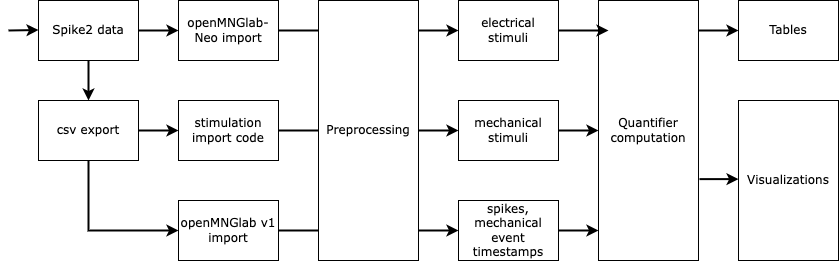
\includegraphics[width = \textwidth]{src/pic/analysis_notebook}
	\caption{Schematic version of analysis pipeline.}
	\label{fig:analysis_notebook}
\end{figure}
\subsubsection{Importing Data}
The first part of the notebook is the import of the data, which consists of two separate importing steps. 
First we use the Neo importer from the current version of our framework to extract the information about the underlying electrical stimulation. After that we use the importer from the old version of openMNGlab to get the spike timings as well as the information about the mechanical stimuli.
After the two importing steps we end up with two separate data structures, that we discussed in the previous chapter, each containing part of the experimental data. From the first importing step, we get the event information about the electrical stimulation in the Neo format. The mechanical stimuli with its physical properties such as amplitude and duration, as well as the spike timings, we receive with the second importing step. This information is contained in the custom data structure. The spike timing would also have been available in the newer Neo format, however, the analysis code was started with the custom data structure in mind, so I did not change that part of the code for the purposes of this thesis. For the future it would be a good idea to switch fully to the Neo structure, so that there is a unified structure for everything.\\
% spike2 csv export to import for additional custom structure
\subsubsection{Preprocressing}
The next part of the notebook contains internal processing steps to sort the spike trains and prepare the data for easy representation and quantification.\\
Making use of the early versions of OpenMNGlab and the first analysis notebooks from Radomir the event plot for the current file gets computed and visualized. The next step is calculating the inter spike distances, meaning the time between two spikes, and creating inter spike distance graphs for each spike train in the recording.\\
\subsubsection{Computing Quantifiers}
Now follows the main part of quantifier computation. This is where the computations of my chosen quantifiers happens. After all the quantifiers are computed the resulting lists of quantifiers for each spike train get put into a data structure and saved for later reimporting and reuse for further analysis.\\
\subsubsection{Visualizations}
Now that the quantifiers are calculated it is time to visualize the results. For this, I created different diagrams showing quantifiers over the whole recording and comparisons of different quantifiers. These figures will be explained in the analysis part of this chapter.\\
%See the appendix for a detailed view of the whole notebook as well as the code.



\section{Spike Analysis}
We have analyzed 22 recording files featuring  mechanical and electrical stimulation. An overview for the data can be found in  Table~\ref{table:recording_overview}. Here we see the number of spike trains in each file and the average spikes per train as well as the average spike train duration. More information about the specific recordings is following in the next section.

%\begin{comment}
\begin{table}[!ht]
\centering
\begin{tabular}{ |c|c|c|c| }
	\hline
	File number & Number of trains  & Avg. spikes per train & Avg. train duration\\
	\hline
	1 & 17 & 12.53 & 0.38 \\
	2 & 34 & 16.62 & 0.39 \\
	3 & 37 & 20.03 & 0.40 \\
	4 & 12 & 4.67 & 0.28 \\
	5 & 11 & 9.18 & 0.25 \\
	6 & 22 & 8.55 & 0.12 \\
	7 & 17 & 10.82 & 0.38 \\
	8 & 16 & 7.38 & 0.40 \\
	9 & 28 & 12.93 & 0.37 \\
	10 & 35 & 8.83 & 0.35 \\
	11 & 37 & 15 & 0.41 \\
	12 & 31 & 13.45 & 0.38 \\
	13 & 18 & 10.28 & 0.24 \\
	14 & 22 & 35.64 & 0.44 \\
	15 & 32 & 13.91 & 0.13 \\
	16 & 32 & 25.53 & 0.39 \\
	17 & 33 & 30.45 & 0.23 \\
	18 & 33 & 29.30 & 0.31 \\
	19 & 31 & 11.74 & 0.38 \\
	20 & 48 & 10.85 & 0.40 \\
	21 & 51 & 22.8 & 0.24 \\
	22 & 50 & 12.16 & 0.36\\
	\hline
\end{tabular}
\caption{This table shows an overview over the available recording files for this thesis.}
\label{table:recording_overview}
\end{table}
%\end{comment}

\subsection{Experimental Protocol}
This subsection will explain how the recording files are structured to get a better general understanding of the experiments and analysis.

As mentioned in previous chapters, the files I am working with feature electrical and mechanical stimulation. The fibers are mechanically stimulated with a custom-built electromechanostimulator~\cite{roberto}. For each fiber the mechanical threshold was determined and then a sufficiently high enough mechanical force was set for the duration of the experiment.
Mechanical force is applied with a duration of 250 or 500 ms, as can be seen in table~\ref{table:recording_overview} with the previously determined force. During their research Uebner et al. found that a sinosoidal stimulus profile works best for the experiments. The attributes of this type of stimulation, like amplitude or duration, is constant over the course of single recordings, but may change  for different recordings. In addition to the mechanical stimulation there is also electrical stimulation, which is applied as electrical impulses with a certain frequency. The base frequency of the electrical stimulation is the same for each of the recordings and lies at $0.1$ Hertz. This base frequency is applied during the whole recording with a few exceptions. Each recording features segments where there is electrical stimulation with increased frequency, during which a varying number of spike trains take place (usually $5-6$). After each of those segments with increased electrical frequency there is a smaller period of stimulation where the frequency is at $0.5$ Hertz before it goes back to the base frequency. One spike train get triggered during each of these small periods. In the recordings that where analyzed in this thesis there are 3 different levels of increased electrical stimulation frequency, which lie at $2.0, 4.0$ and $5.0$ Hertz.\\
Each file features at least one burst of increased frequency at one of the mentioned levels. The files in Table~\ref{table:recording_overview} are ordered according to the frequencies of electrical stimulation that occurred in the recordings. Files $1-3, 4-12, 13-14$ contain only frequencies of $2.0, 4.0, 5.0$ Hertz respectively. Files $15-20$ contain both $2.0$ and $4.0$ Hertz frequencies and files $21-22$ contain all three types of increased frequencies.\\

\subsection{Sample Analysis}
To show the results of the analysis in more detail I will use recording 21 as an example and demonstrate the outcomes. This will give a good look at the quantifiers that I chose to utilize as well as present possible visualizations using those quantifiers.

\subsubsection{Table of Values}
When applying the analysis notebook to a recording, the first basic output we get is a big table containing the finished quantifiers as well as the original timestamp values for the spikes. A sample table can be seen in Table~\ref{fig:table_sc}, which shows a screenshot of the output table for recording 21.
First of all the table contains the mechanical stimulus information for each train. This includes the amplitude, duration and timestamp of the corresponding stimulus. In the figure this information is contained in the upper third of the table.
In addition the table features the single value quantifiers for the spike trains that I described in the previous chapter. These include among others the peak firing frequency, spike count and mean firing frequency and can be found in the middle third of the figure.
Lastly the table also features some of the raw data such as the spike timings as well as some intermediate results such as the inter pike intervals, which can be used to compute some of the single value quantifiers. These are depicted in the lower third of the figure in an abbreviated version for the sake of visibility.\\
\begin{figure}
	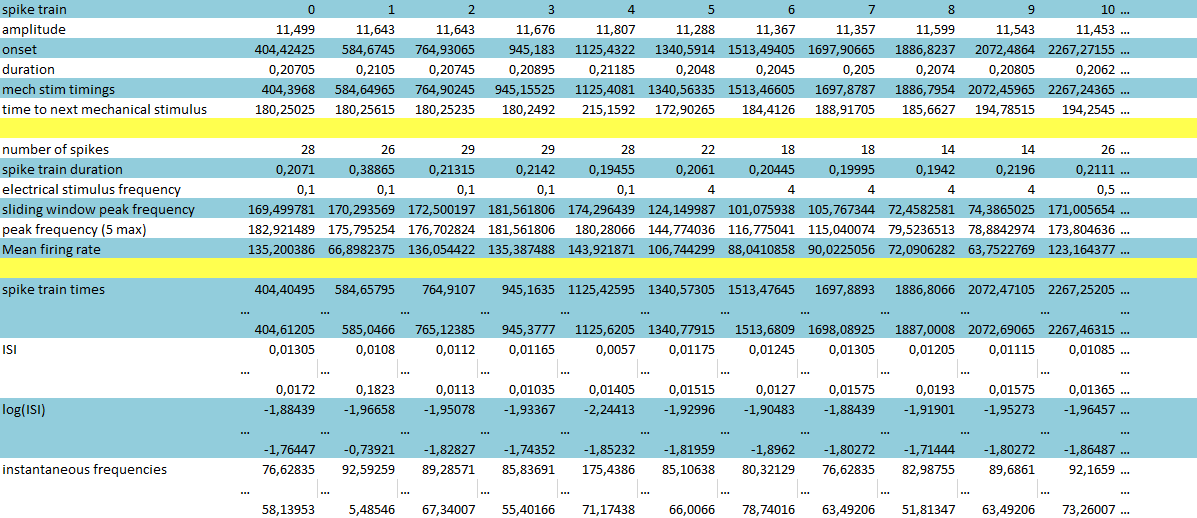
\includegraphics[width = \textwidth]{src/pic/sc_table}
	\caption{Sample picture of table after successful analysis }
	\label{fig:table_sc}
\end{figure}




\subsubsection{Comparative Diagrams for Quantifiers}
Having computed the quantifiers is all well and good, but now we want to visually compare them in order to see if there is correlation between them in any way.
\begin{figure}
	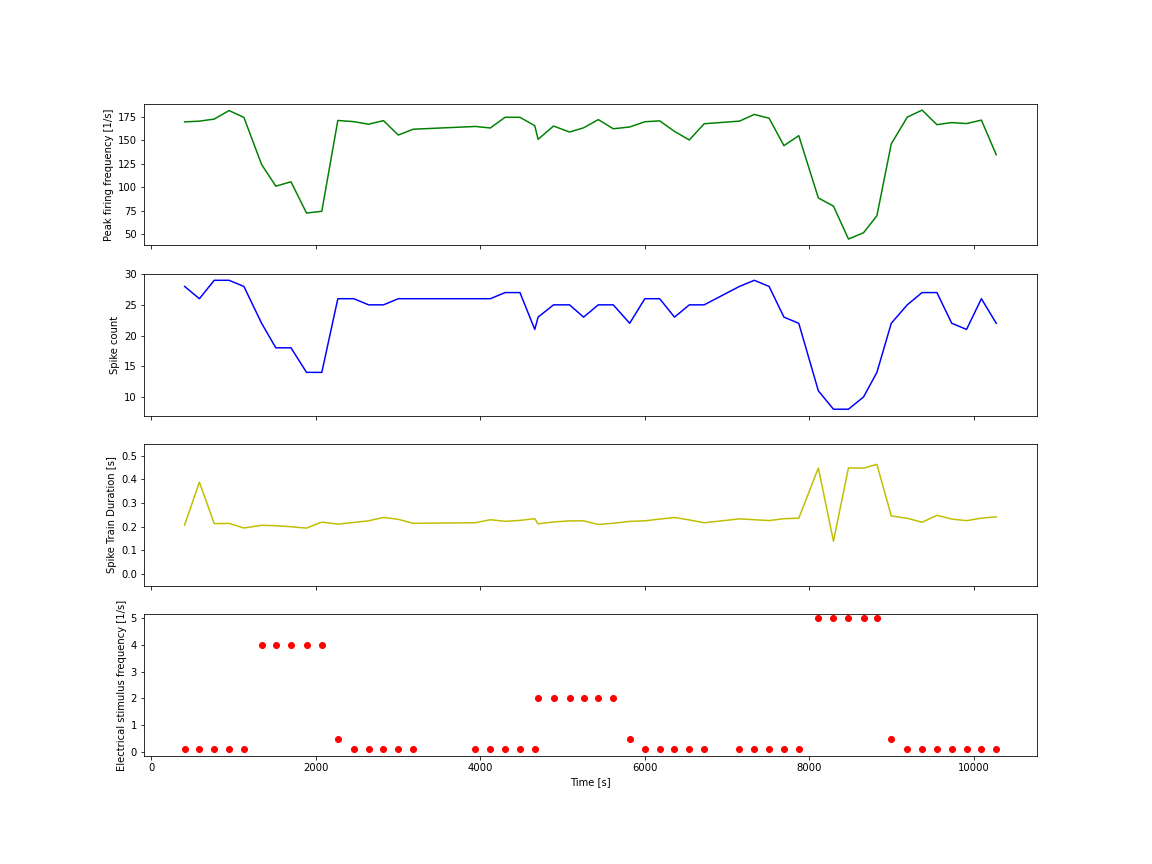
\includegraphics[width = \textwidth]{src/pic/11_12_13_sp}
	\caption{Diagram showing a separated comparison of peak firing frequency and spike count for recording 21}
	\label{fig:quantcomp_sp}
\end{figure}
\begin{figure}
	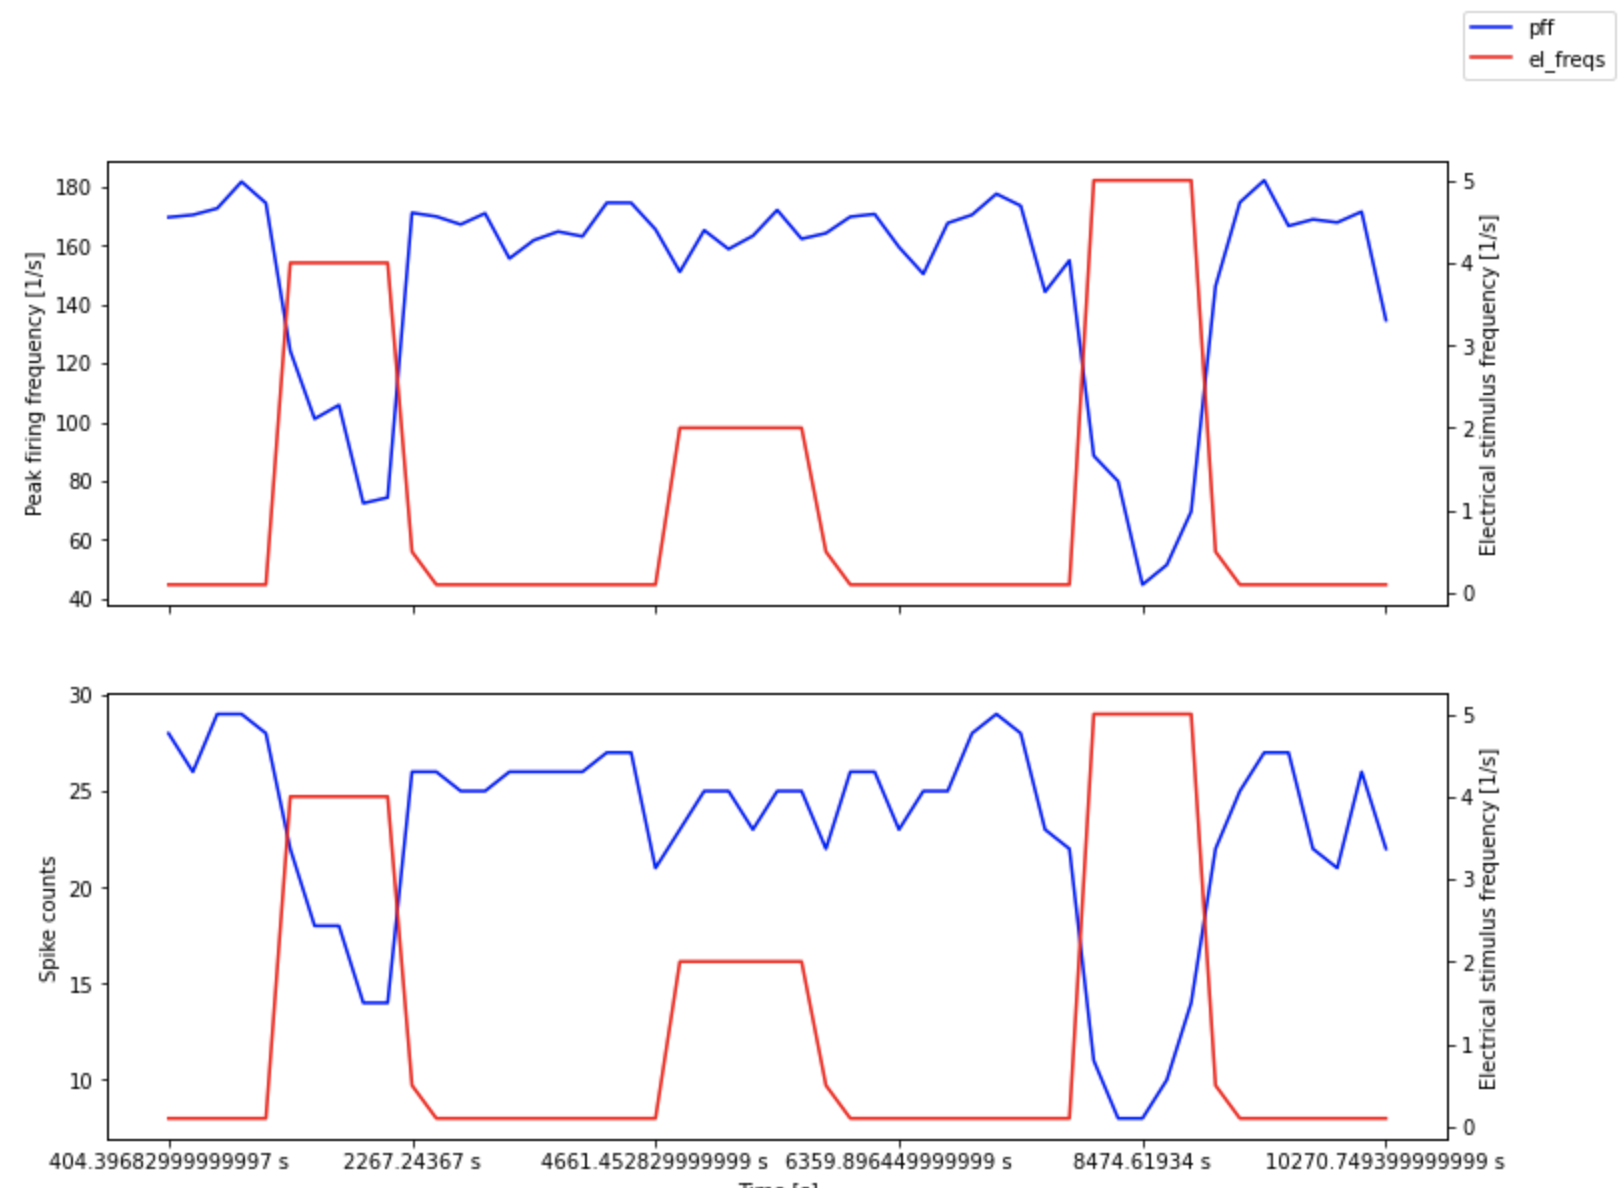
\includegraphics[width = \textwidth]{src/pic/11_12_13_cm}
	\caption{Diagram showing a comparison of peak firing frequency and number of spikes for recording 21}
	\label{fig:quantcomp_cm}
\end{figure}

A good visualization of this can be seen in figure~\ref{fig:quantcomp_sp}. This figure compares the spike count with the Peak firing frequency in recording 21. The time is plotted on the x axis ranging from the start of the recording to the end. This recording lasted over 10000 seconds. For each spike train we plotted the Peak firing frequency, the spike count as well as the Spike train duration in separate rows of the figure. In addition we added the electrical stimulation frequency, to see what effect the changes in frequency have on different quantifiers. Figure~\ref{fig:quantcomp_cm} shows the same data in a slightly different format. Here the electrical stimulation frequency is included in the rows where we plot the quantifiers to better see the immediate effect.\\
The first thing that we can observe is that the Peak firing frequency and spike count behave very similarly and have almost the exact same graph. Secondly, the application of different electrical stimuli does seem to have an effect on the spike trains. We can see that in the areas with 4 and 5 Hertz stimulation the peak firing frequency as well as the spike count take a significant dip. However, the same cannot be said for the interval with 2 Hertz stimulation. The quantifiers stay largely the same, which leads us to the assumption that there is some sort of threshold which needs to be passed in order to influence the spike trains. In our recordings this threshold seems to lie somewhere between the 2 and 4 Hertz electrical stimulation marks.
While the peak firing frequency and spike count show significant variation, the pike train duration stays pretty constant for the 4 Hertz stimulation but does also increase during 5 Hertz stimulation. This may point to different thresholds for different aspects of a spike train.

\subsubsection{Instantaneous Frequencies}
\begin{figure}
	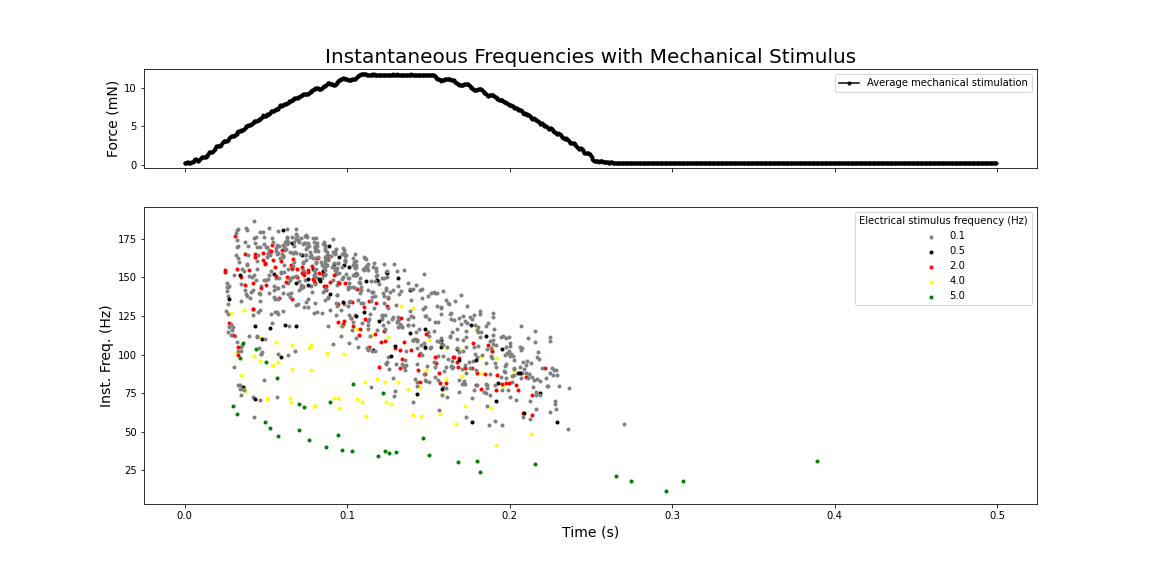
\includegraphics[width = \textwidth]{src/pic/11_12_13U1b_inst_freqs}
	\caption{Figure showing the instantaneous frequencies in each spike train for one recording.}
	\label{fig:inst_freqs}
\end{figure}
Another quantifier that we can take a look at is the instantaneous frequencies of the spikes in the spike trains and observe how these change with different levels of electrical stimulation. To visualize this we recreated a figure from the original paper from Roberto de Col in figure \ref{fig:inst_freqs}. The data for this figure is taken from recording 21. The x axis depicts the time since the last stimulus in seconds. The top part of the figure shows the force of mechanical stimulation that evoke the spike trains. This curve represents the average mechanical stimulus in this recording. A sliding window of three was used for the calculation of the instantaneous frequencies to smooth out some of the outliers. The lower part of the figure is a scatterplot of these instantaneous frequencies for every spike train in the recording. They were color-coded according to the underlying electrical stimulation frequency. The pike trains with the base level frequency of 0.1 Hertz are colored in gray, while the trains with higher stimulation are colored in red, yellow and green for an electrical frequency of 2, 4 and 5 Hertz respectively. Finally the trains with a stimulation of 0.5 Hertz stimulation frequency are colored in blue. From the scattering of the dots we can observe that the spike trains occurring during an electrical stimulation of 4 and 5 Hertz show lower instantaneous frequencies than the base level spike trains. The red dots lie mostly in the main cluster of dots belonging to the base level spike trains, which would fit with the previous figures and the assumption of some sort of threshold for spike train alterations.

\subsubsection{Event plot}
A figure that we have seen previously in this chapter is the event plot. It shows an overview of spiking activity after mechanical stimuli over the course of a whole recording. Figure~\ref{fig:event_color} shows a color coded event plot. This shows the same recording as figure~\ref{fig:inst_freqs} and uses the same color coding for the electrical frequencies. It is not meant to be an in depth analysis tool, but rather a quick visual representation of a recording. This can give us an idea if it makes sense to further analyze a particular recording, by looking at the length of the spike trains.

\begin{figure}
	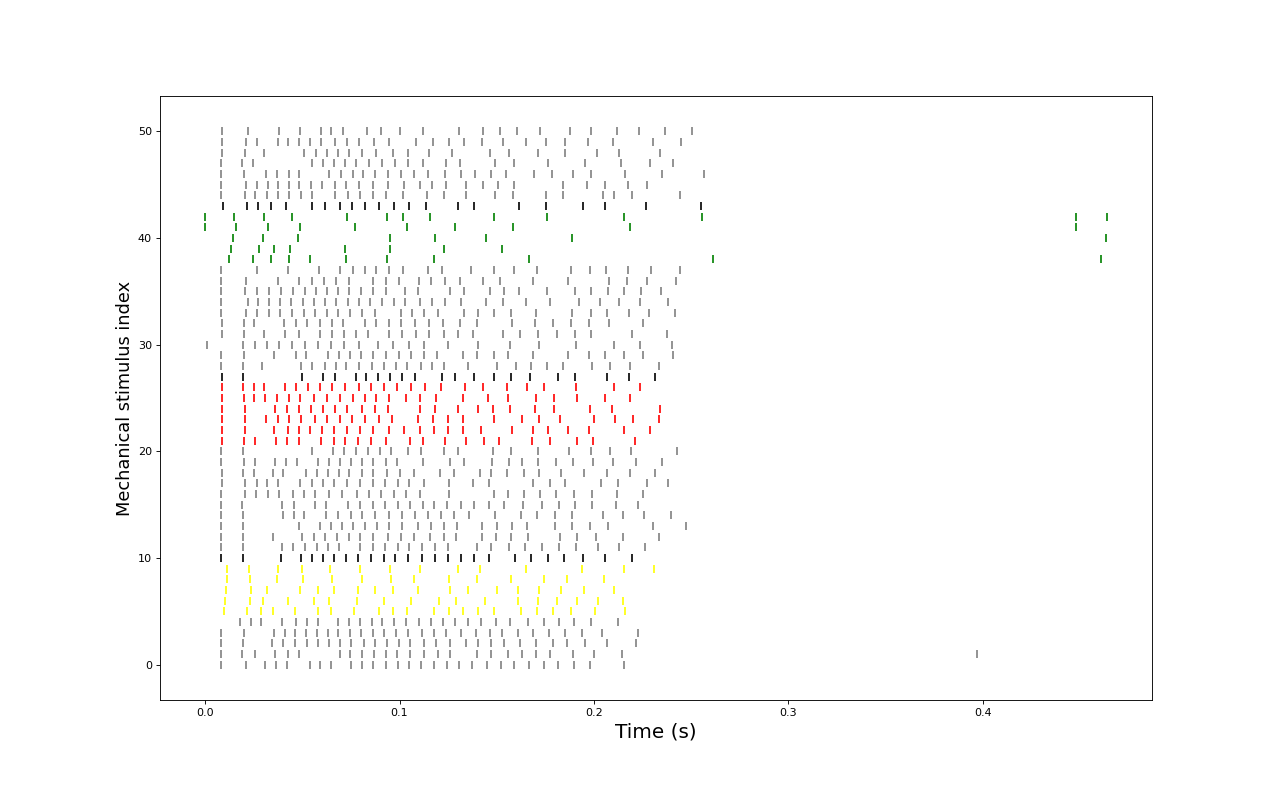
\includegraphics[width = \textwidth]{src/pic/11_12_13U1bevent_color}
	\caption{Color coded event plot}
	\label{fig:event_color}
\end{figure}



%-diagrams of Interspike Intervals(isi) and logarithm of isi\\
%-should show that by taking the logarithm, the isi becomes more linear\\




\cleardoublepage
